\documentclass[a4paper,fleqn]{cas-sc}

 %\usepackage[numbers]{natbib}
%\usepackage[authoryear]{natbib}
%\usepackage[authoryear,longnamesfirst]{natbib}
\usepackage{float}
\usepackage{svg} 
\usepackage[utf8]{inputenc}
%\usepackage{fontspec}
%\newfontface{\bn}{kalpurush.ttf} 
\usepackage[numbers]{natbib}
\usepackage{tabularx}
\usepackage[english]{babel} 
\usepackage{algorithm} 
\usepackage{algpseudocode}
\usepackage{lineno}
\usepackage{amsmath}
\usepackage{amsfonts}
\usepackage{amssymb}
\usepackage{algpseudocode} 
\usepackage{booktabs}
\usepackage{multirow} 
\usepackage{changepage} 
\usepackage{orcidlink}
\usepackage{hyperref}
\usepackage{subcaption}
\usepackage{color}
\usepackage{xcolor} 
%%%Footer and ORCID adjustments
% This is a preprint, not a submitted manuscript: drop the "submitted to Elsevier" wording.
\ExplSyntaxOn
\cs_set:Npn \__first_footerline:
  {
    \group_begin:
    \small
    \sffamily
    \ifnum\theblind>0\relax
    \else
    \__short_authors: :~
    \fi
    \rmfamily \itshape Preprint
    \group_end:
  }
\ExplSyntaxOff
% No ORCID identifiers are used, so hide the empty ORCID footnote.
\RenewDocumentCommand \printorcid { } { }
%%%Author definitions
\def\tsc#1{\csdef{#1}{\textsc{\lowercase{#1}}\xspace}}
\tsc{WGM}
\tsc{QE}
\tsc{EP}
\tsc{PMS}
\tsc{BEC}
\tsc{DE}
%%%
%\rightlinenumbers*
\begin{document}
\let\WriteBookmarks\relax
\def\floatpagepagefraction{1}
\def\textpagefraction{.001}

% Short title
\shorttitle{Trust-Calibrated Multi-Agent Scientific Deliberation for Mitigating Sycophantic Consensus}

% Short author
\shortauthors{Rahaman et~al.}

% Main title of the paper
\title [mode = title]{Trust-Calibrated Multi-Agent Scientific Deliberation for Mitigating Sycophantic Consensus in LLM Reasoning} 


\author[1]{Md. Atikur Rahaman}
\cormark[1]
\ead{mrahaman2310298@bscse.uiu.ac.bd}
\credit{ Conceptualization, Formal analysis,  Methodology, Writing-original draft, Writing-review \& editing}
% Address/affiliation
 \affiliation[1]{organization={Computer Science and Engineering, United International University},
    %addressline={}, 
    city={Dhaka},
    citysep={}, % Uncomment if no comma needed between city and postcode
    postcode={1212}, 
    %state={E Wesley Ave, Denver},
    country={Bangladesh}}

% Second author
\author[1]{Rakibul Hasan}
\ead{rhasan2310530@bscse.uiu.ac.bd}
\credit{Conceptualization, Data curation, Formal analysis, Methodology, Validation}

% Third author
\author[1]{Md. Salman Rohoman Nayeem}
\ead{salmanrahman339@gmail.com}
\credit{Data curation, Investigation, Software, Writing - review \& editing}

% Fourth author
\author[1]{Pratay Paul}
\ead{ppaul2310163@bscse.uiu.ac.bd}
\credit{Data curation, Software, Validation, Visualization}

% Fifth author
\author[1]{Yousuf Kamal Himel}
\ead{yhimel2310526@bscse.uiu.ac.bd}
\credit{Data curation, Formal analysis, Validation, Writing - review \& editing}

% Sixth author
\author[1]{Mst. Farjana Akter Limu}
\ead{mlimu2310535@bscse.uiu.ac.bd}
\credit{Data curation, Software, Validation, Visualization}

% Supervisor
\author[1]{Mohammad Nurul Huda}
\credit{Investigation, Supervision, Visualization}

% FYDP faculty
\author[1]{Ohidujjaman}
\credit{Supervision, Validation, Writing - review \& editing}

\cortext[cor1]{Corresponding author: Md. Atikur Rahaman (mrahaman2310298@bscse.uiu.ac.bd)}
 
% Here goes the abstract
\linenumbers 
\begin{abstract}
   Large language models have done surprisingly well at answering many scientific questions. However, large language models also continue to "hallucinate" and reason incorrectly. One potential solution to these problems is multi-agent debate. Although a correct minority may exist, a confident but incorrect majority can drag this correct minority agent down and lead the group to select the wrong answer. This is known as the "sycophantic consensus." Currently, there is no mechanism within any debate system to check an individual agent's assertions against outside scientific evidence before allowing them to gain influence in the debate. Instead of using a simple vote-weighted approach, we intend to assign a trust score to every participating agent based on how much scientific evidence supports their responses. Every time agents respond during a round, the system breaks down their responses into small units of factually verifiable statements ("claims"). After breaking down the response, the system locates all relevant scientific literature that could support or contradict each claim. Because unsupported claims eventually lose influence and because the trust scores are kept in bounds, the probability increases that a correct minority will survive long enough to ultimately win. Our proposed framework produced fewer hallucinated answers than competing frameworks because all surviving claims are linked back to their originating passages of scientific evidence. To test this hypothesis, we compare our proposed framework to majority voting and other baseline systems. Once all models have finished responding to a given question, the system returns both the selected model and supporting citations for that model. The performance of our proposed framework is evaluated via four metrics: answer accuracy, consensus collapse, minority preservation, and evidence calibration.

\end{abstract}
% Keywords
% Each keyword is separated by \sep
\begin{keywords}
 Large language models \sep Multi-agent debate \sep  Retrieval-augmented generation \sep  Sycophancy \sep Scientific question answering \sep Trust calibration 
\end{keywords}

\maketitle
\linenumbers  
\section{Introduction}\label{sec1}

Large language models can answer scientific questions at a level that makes them useful for tutoring and decision support. A model can still be confidently wrong, and it can state a wrong answer in fluent language that hides the error. Multi-agent debate reduces this risk because three agents answer the same question and review each other's reasoning over rounds~\cite{du2024improving}. Chain-of-thought prompting lets each agent expose the steps behind its answer, so peers can inspect the reasoning~\cite{wei2022chain}. The weak point sits at the end of the debate. Most systems combine the answers by majority vote, where every agent counts the same and the most frequent answer wins~\cite{wang-etal-2024-rethinking-bounds,choi2025debate}. A confident and wrong majority can then push a correct minority agent to drop its answer, and the vote records the wrong result as agreement. This failure is called sycophantic consensus~\cite{pitre-etal-2025-consensagent,he2026minority}. No current debate system checks an agent's claims against outside scientific evidence before that agent earns influence. This study builds a trust-calibrated multi-agent deliberation framework to close that gap. Each agent's answer is split into small factual claims. The claims are checked against retrieved scientific literature, and every agent holds a bounded trust score that rises with supporting evidence and falls with contradicting evidence. The final answer comes from trust-weighted aggregation instead of a head count. The method is tested on scientific reasoning datasets such as GPQA and MMLU-Pro, and it needs no fine-tuning because all models run as served inference.

Du et al. show that debate improves factuality and reasoning over a single pass, but their agents are treated equally and their claims are never checked against external sources~\cite{du2024improving}. Pitre et al. report that the correct answer is present in the discussion yet ignored in more than 20 percent of wrong-answer cases, and their prompt-rewriting fix still leaves the final decision on self-reported confidence~\cite{pitre-etal-2025-consensagent}. The uncertainty route of Yoffe et al. reweights agent influence during the debate, and their own ground-truth experiment shows the gain is capped by the quality of that self-reported signal~\cite{yoffe-etal-2025-debunc}. Token cost is the target of Fan et al., who decide when a debate is worth running, yet majority voting remains once the debate starts~\cite{fan2026imad}. Wang et al. combine many models through static aggregation and score well on open benchmarks, with no per-agent trust and no evidence check~\cite{wang2025mixture}. He et al. detect a suppressed correct minority after the debate and overturn the majority, which comes too late to protect the minority while it argues~\cite{he2026minority}.

Across these systems, influence is set by a vote, a self-reported score, a prompt rewrite, or a post-hoc flip, and none of them verifies an agent's claims against evidence while the debate is running. Self-reported confidence is a weak basis because training that makes models agreeable also makes them more sycophantic and less accurate~\cite{ibrahim2026training}, and alignment training has been shown to increase agreement with wrong user positions~\cite{chen2025self}. Theory also predicts that correlated agents drift to a wrong majority unless an outside correction enters the loop~\cite{estornell2024multillm}, and multi-agent systems fail in recurring ways that diagnosis alone does not fix~\cite{cemri2025why}. This study resolves the unsolved part by tying each agent's influence to external evidence during the debate. Claims are checked against retrieved passages from scientific sources~\cite{karpukhin2020dense,kushwaha2026agentbased}, a step in line with work that grounds correction in external tools~\cite{gou2024critic}. The trust score is bounded, so no agent is silenced or made all-powerful, and the final decision uses those weights. Scientific question sets are a suitable testbed because they carry verifiable answers and published literature that retrieval can reach, and GPQA and MMLU-Pro allow comparison against established baselines. The expected outcome is a reproducible framework that lowers consensus collapse, preserves a correct minority more often, keeps answer accuracy stable, and reports a calibrated trust signal.

%%%%%%%%%%%%%%%%%%%%%%%%%%%%%%%%
\section{Conventional Method}\label{sec2}

\subsection{Preliminaries}
Large language models can answer many scientific questions, but they still produce confident errors. Chain-of-thought prompting makes the reasoning path visible, so a reader can follow the steps that produced an answer~\cite{wei2022chain,zhang2025from}. Multi-agent debate extends this idea. Several agents answer the same question, read the reasoning of the other agents, and revise their positions over rounds before a final answer is selected~\cite{du2024improving}. The combination step is as important as the reasoning itself. Most debate systems combine the answers with a majority vote, and every agent carries the same weight in that vote~\cite{wang-etal-2024-rethinking-bounds}. A majority vote counts repeated answers. It does not check whether an answer is correct. A confident but wrong majority can push a correct minority agent to change its answer, and the vote records the wrong result as agreement. This behavior is called sycophantic consensus~\cite{pitre-etal-2025-consensagent}. Debate systems usually rely on two confidence signals, namely self-reported confidence and token-level uncertainty. Neither signal checks the truth of the claim that carries it~\cite{yoffe-etal-2025-debunc}. Trust in a debate answer therefore has to come from evidence outside the debate.

\subsection{Existing Methods}
Existing research lines address parts of this problem. Du et al. show that debate improves factuality and reasoning over a single pass, but their agents are treated equally and their claims are never checked against external sources~\cite{du2024improving}. Fan et al. reduce the cost of debate by predicting when a debate is worth running, and the aggregation step remains a majority vote once the debate starts~\cite{fan2026imad}. Wang et al. combine model outputs through a layered pipeline and report strong results on open benchmarks, with no per-agent trust and no evidence check~\cite{wang2025mixture}. Zhou et al. choose specialized reasoners for subtasks through a reward-driven process, which selects who works on a task but not how much each answer counts~\cite{zhou2025reso}.

A second group of methods targets sycophancy directly. Pitre et al. report that the correct answer is present in the discussion but ignored in more than 20 percent of wrong-answer cases. Their framework detects stalling or answer copying, rewrites the task prompt, and restarts the debate, while the final vote still uses self-reported confidence~\cite{pitre-etal-2025-consensagent}. Chen et al. reduce sycophancy through preference alignment at training time, which operates on one model and does not cover a live debate~\cite{chen2025self}. Ibrahim et al. show that training models to sound warm lowers factual accuracy and raises agreement with false user beliefs~\cite{ibrahim2026training}. He et al. detect a suppressed correct minority after the debate and flip the majority decision, which comes too late to protect the minority during the rounds~\cite{he2026minority}.

A third group changes the information that agents receive. Yoffe et al. reweight agent influence during the debate with token-level uncertainty, and their ground-truth experiment shows that the gain is limited by the quality of that internal signal~\cite{yoffe-etal-2025-debunc}. Gou et al. ground correction in external tools for a single agent~\cite{gou2024critic}. Kushwaha and Madhavan detect contradictions between retrieved documents and score source credibility before generation, without a debate between agents~\cite{kushwaha2026agentbased}. Karpukhin et al. provide the dense passage retrieval method that this study adopts for its retrieval stage~\cite{karpukhin2020dense}.

Theory and diagnosis complete the picture. Estornell and Liu prove that similar responses cause majority tyranny and that shared misconceptions lower accuracy as more agents share them~\cite{estornell2024multillm}. Choi et al. separate debate from voting and show that majority voting explains a large part of the reported gain~\cite{choi2025debate}. Cui et al. remove the consensus requirement and score the debate trajectory instead~\cite{cui2026freemad}. Pitre et al. evaluate debate process quality when ground truth is unavailable~\cite{pitre2026diagnostic}. Cemri et al. build a failure taxonomy for multi-agent systems and report failure rates between 41 and 86.7 percent across seven systems, and they leave correction to future work~\cite{cemri2025why}. Cau et al. show that selective persuasion drives agreement, and Yeow et al. show that feedback between agents can spread early errors~\cite{cau2025selective,yeow2025reliable}.

\subsection{Research Gap}
Three issues remain open in multi-agent debate. The first issue is the cost of a debate. iMAD predicts whether a debate is needed before it starts, which lowers the token cost on easy questions~\cite{fan2026imad}. The second issue is how to detect agreement that comes from conformity or sycophancy. CONSENSAGENT detects stalling and answer copying, and it rewrites the prompt before the next round~\cite{pitre-etal-2025-consensagent}. The third issue is how to decide which agent should carry more influence when the agents disagree. DebUnc weights agent influence with self-reported uncertainty, and its own diagnostic ground-truth experiment shows that the weighting mechanism works only as well as the uncertainty signal it receives~\cite{yoffe-etal-2025-debunc}.

Existing fixes do not close the third issue. Static aggregation treats every proposer the same and leaves the synthesis to one model, so a confidently wrong proposer enters the final answer on equal footing~\cite{wang2025mixture}. Process-level diagnosis measures the health of a debate but does not change the decision~\cite{pitre2026diagnostic}. A post-hoc flip protects a suppressed minority after the debate ends, when the pressure on that minority has already happened~\cite{he2026minority}. Tool-based correction verifies one agent's output in isolation, and it does not arbitrate between agents~\cite{gou2024critic}. Retrieval-side credibility scoring ranks sources before a single generation pass, with no revision rounds and no agent trust~\cite{kushwaha2026agentbased}. Theory predicts that correlated agents drift to the majority regardless of correctness and that shared misconceptions lower accuracy as more agents share them~\cite{estornell2024multillm}. Training-time work shows that alignment can make this tendency stronger, because models trained to sound agreeable grow more sycophantic and less accurate~\cite{ibrahim2026training,chen2025self}. Empirical studies of failure also show that these failures are recurring and classifiable, and they leave correction to future work~\cite{cemri2025why}. Debate-only baselines confirm that voting carries much of the reported gain, and voting is the component that cannot separate a correct answer from a repeated one~\cite{choi2025debate}.

Across the reviewed work, influence is set by a vote, a self-reported score, a prompt rewrite, or a post-hoc flip. No method verifies an agent's claims against external evidence while the debate is running, and no method uses such a verification to set the weight of that agent in the final decision. This study fills that gap with a bounded trust score that is updated from retrieved evidence during the debate and used for the final aggregation.

\section{Proposed Method}\label{sec3}

\subsection{Framework Overview}
The framework is a deliberation layer that sits between a scientific question and its final answer. A question first passes the confidence gate. The gate chooses between a direct answer and a full debate. Inside a debate, three heterogeneous agents answer the question independently and tag the claims in their reasoning. Each claim is checked against retrieved scientific evidence. The verdicts update the trust score of every agent, and the agents revise their positions with the peer answers and their own trust standing in view. The loop runs for at most three rounds. The final answer is selected by a trust-weighted aggregation over the agent positions. The result package contains the answer, the supporting citations, the trust trajectory, and the reasoning trace of each agent. Figure~\ref{fig:framework-flow} shows the end-to-end flow, and Figure~\ref{fig:context} shows the system boundary and the external actors.

\begin{figure}[pos=htbp]
  \centering
  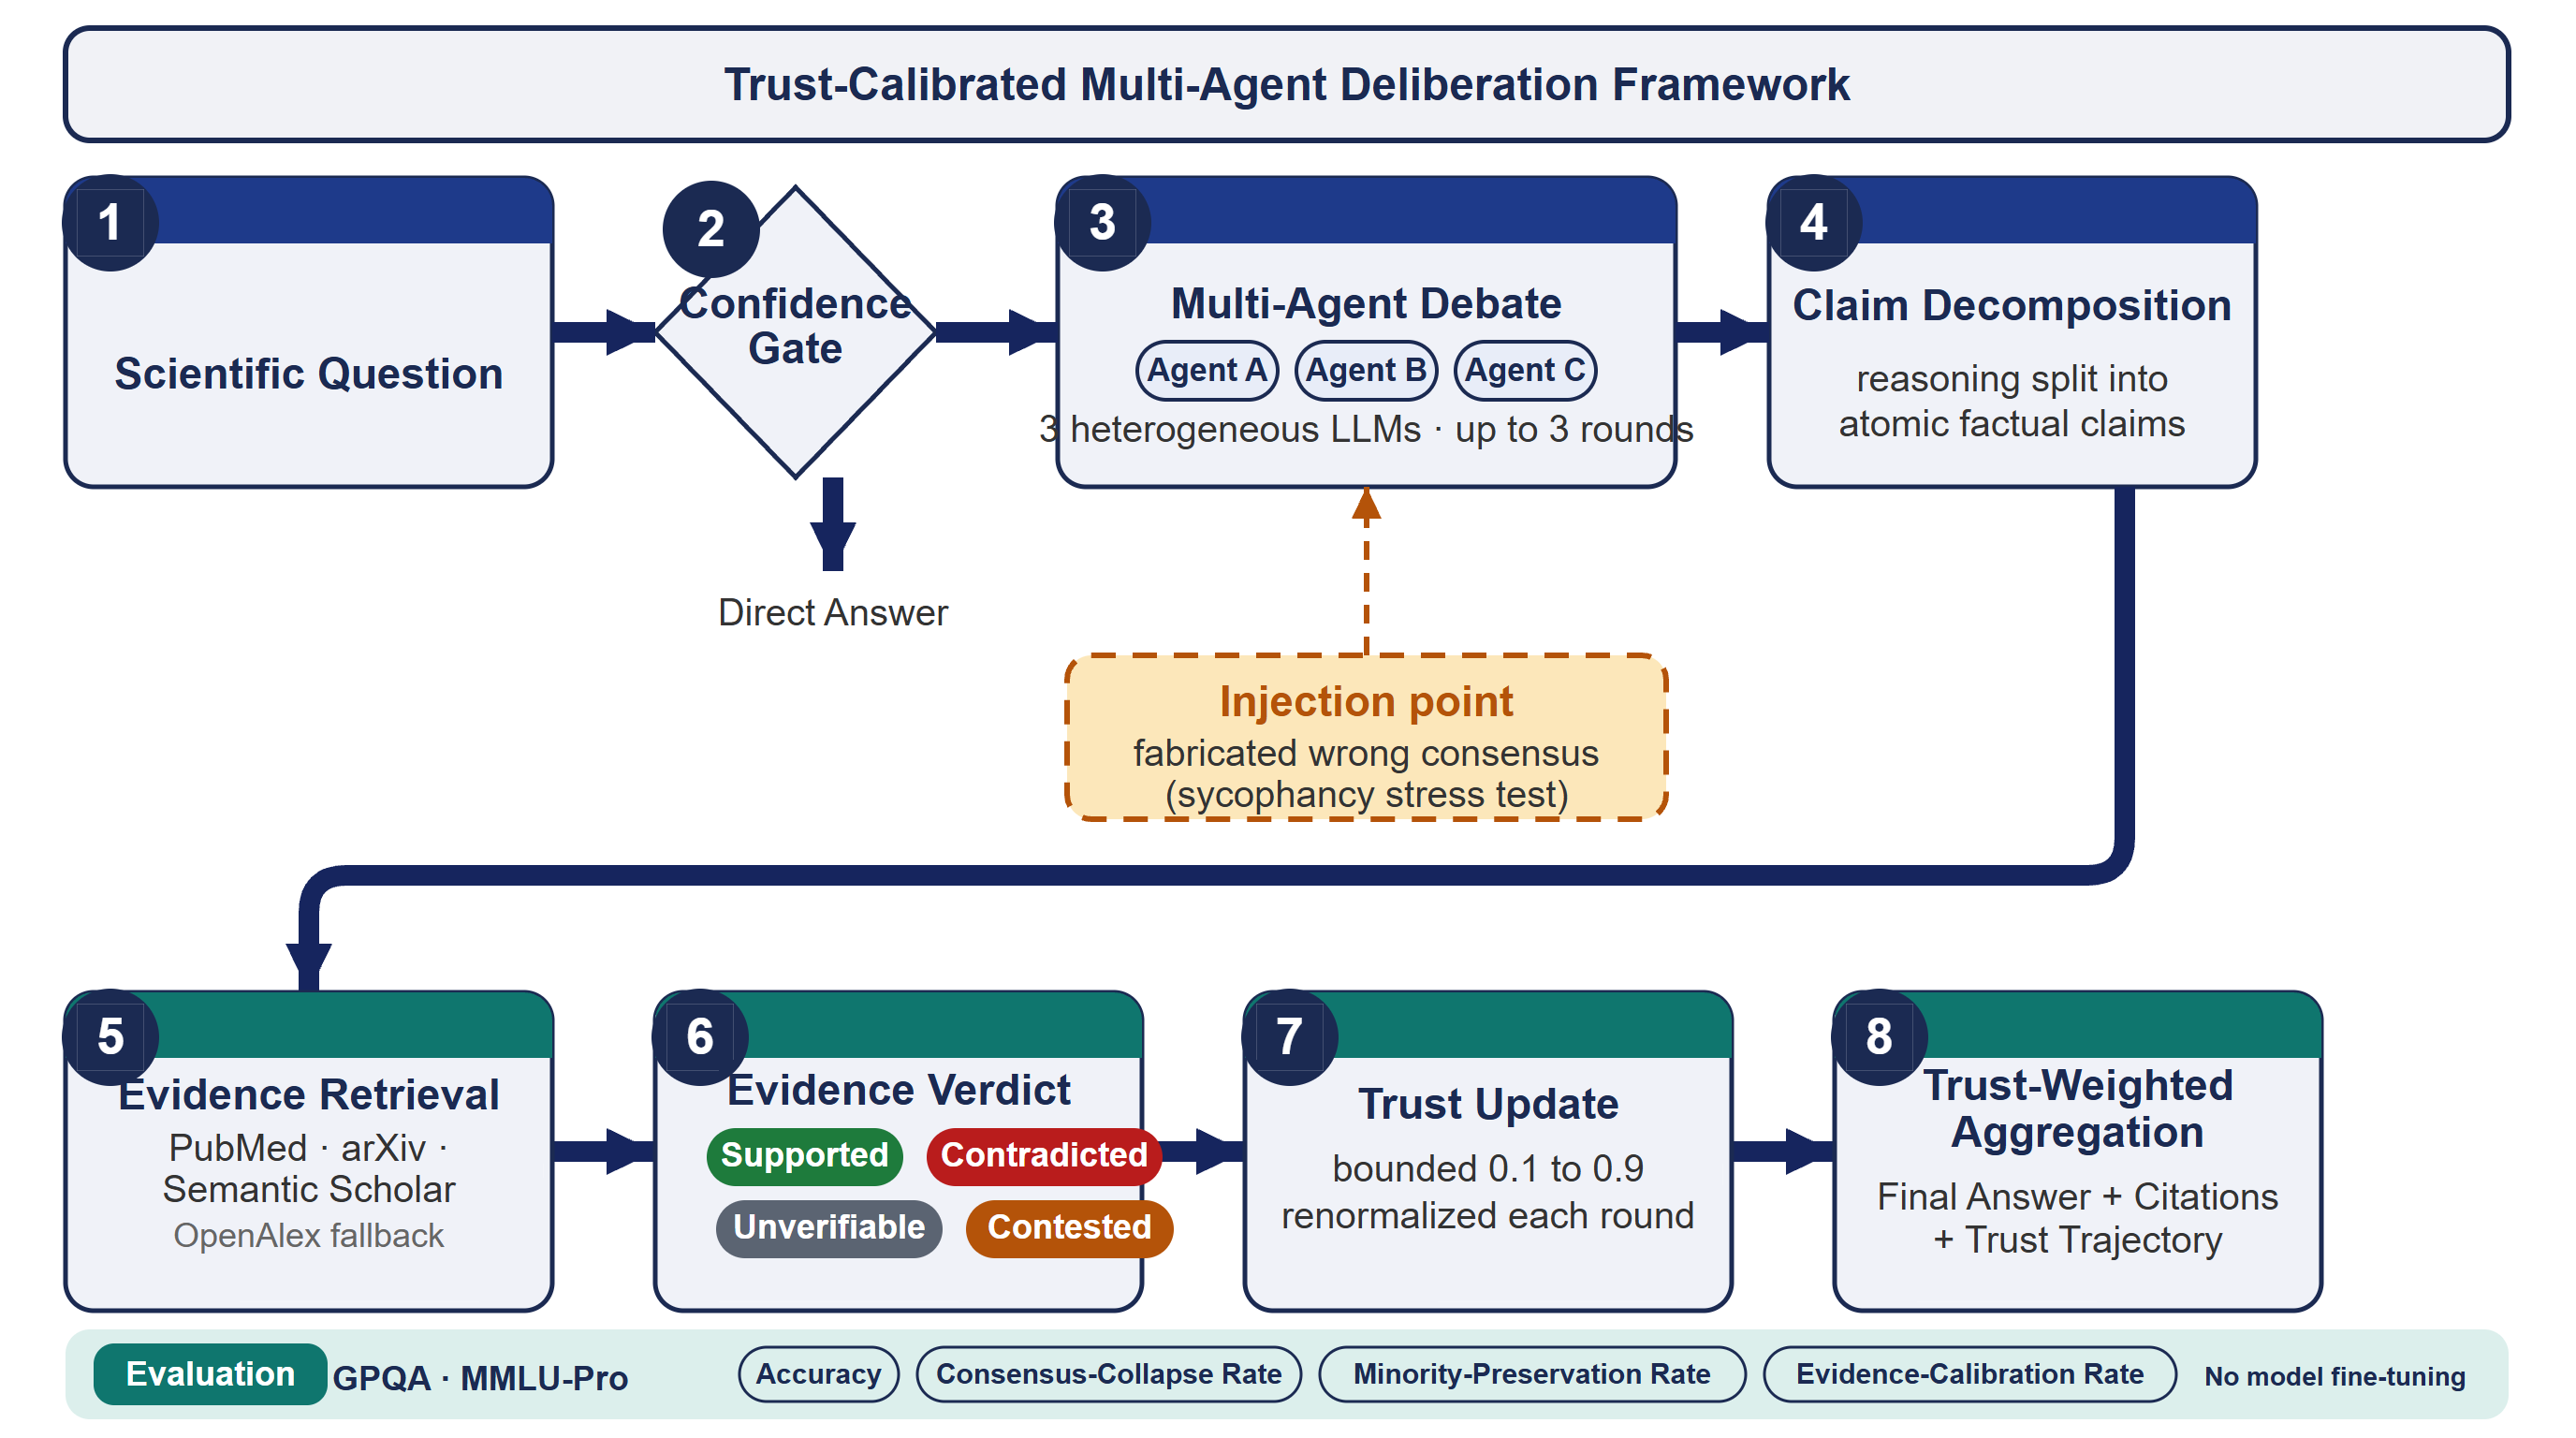
\includegraphics[width=0.88\linewidth]{fig-pipeline.png}
  \caption{End-to-end flow of the trust-calibrated multi-agent deliberation framework: debate, claim-level evidence verification, per-round trust updates, and trust-weighted aggregation.}\label{fig:framework-flow}
\end{figure}

\begin{figure}[pos=htbp]
  \centering
  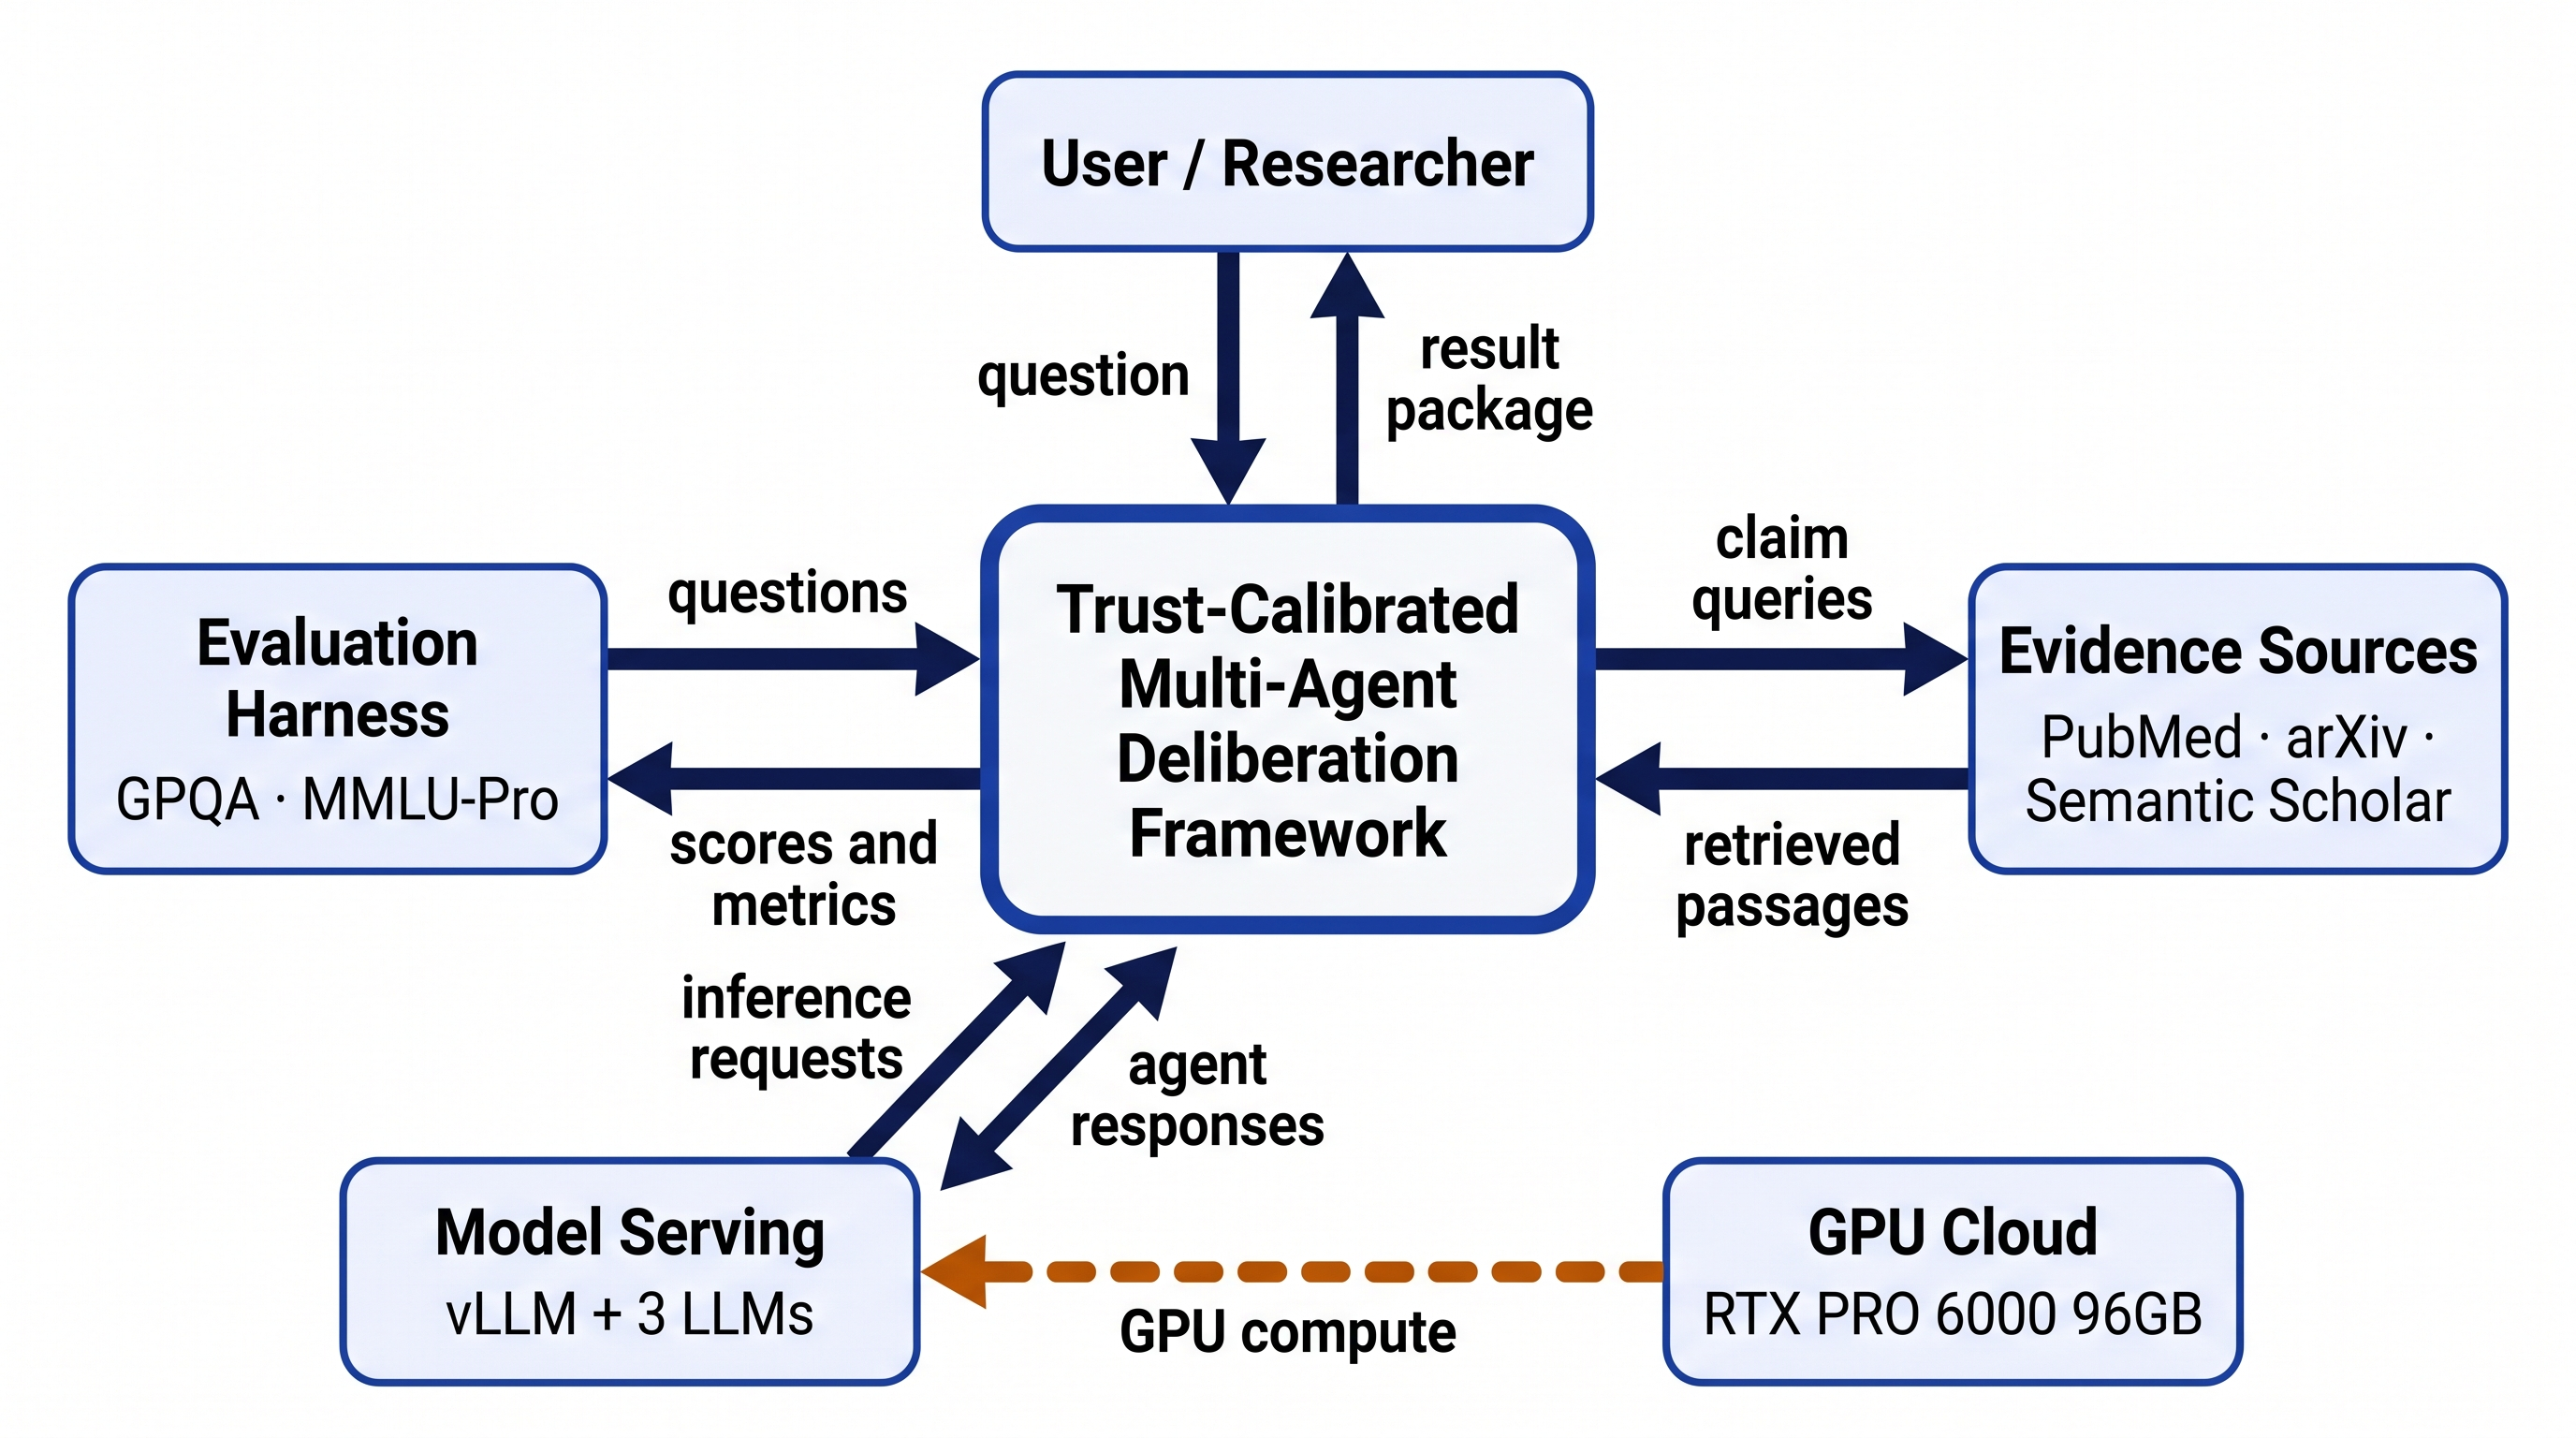
\includegraphics[width=0.80\linewidth]{fig-context.png}
  \caption{Context diagram of the framework. The evaluation harness submits questions, the evidence sources return passages, the model server runs the three agents, and the user receives the result package.}\label{fig:context}
\end{figure}

\subsection{Confidence Gate}
The gate keeps the cost low on easy questions. One agent answers the question with a short chain of thought and reports a confidence value, or three quick agent calls answer the same question and the gate compares the answers. A low confidence or a disagreement sends the question to the full pipeline. A high confidence sends the question to a direct answer. The gate affects throughput and not the core evaluation, because the evaluation set keeps only questions that produce divergent initial answers.

\subsection{Heterogeneous Debate Agents}
Three agents answer the question in round zero. Each agent is a different model family, so the agents do not share the same training data and the same blind spots~\cite{estornell2024multillm}. The development configuration uses Qwen3.5-9B, Gemma 4 12B, and Ministral-3-14B-Instruct-2512. The final configuration replaces them with Qwen3.6-27B, Gemma 4 26B A4B, and Mistral-Small-3.2-24B-Instruct-2506. All models are served through vLLM behind an OpenAI-compatible interface, and no model is fine-tuned. Each agent produces an answer, a reasoning trace, and a list of tagged claims in the form \texttt{<claim id="c1">}. The tags make claim-level checking possible in later stages.

\subsection{Claim Decomposition}
A compound sentence can carry more than one fact. The decomposition step splits each agent answer into small factual statements, and every statement keeps the identifier of its source agent. A schema check validates the tagged output. A failed check triggers a fallback extraction pass that recovers the claims from the raw text. A claim that no source can verify is marked unverifiable and is excluded from the trust update, so an abstention neither rewards nor penalizes the agent.

\subsection{Source-Partitioned Retrieval and Evidence Scoring}
The three agents do not share one retrieval source. Agent one sends its claims to PubMed, agent two to arXiv, and agent three to the Semantic Scholar Graph API. OpenAlex is the fallback when a source is unavailable, and retrieved results are cached so repeated runs do not hit rate limits. A cross-encoder reranker scores each claim against the retrieved passages and keeps the highest scoring passages~\cite{karpukhin2020dense}. Every claim then receives one of four verdicts, namely supported, contradicted, unverifiable, or contested. A claim with conflicting high-score passages is marked contested and reported separately in the evaluation. Figure~\ref{fig:claim-example} shows one claim checked against a retrieved passage.

\begin{figure}[pos=htbp]
  \centering
  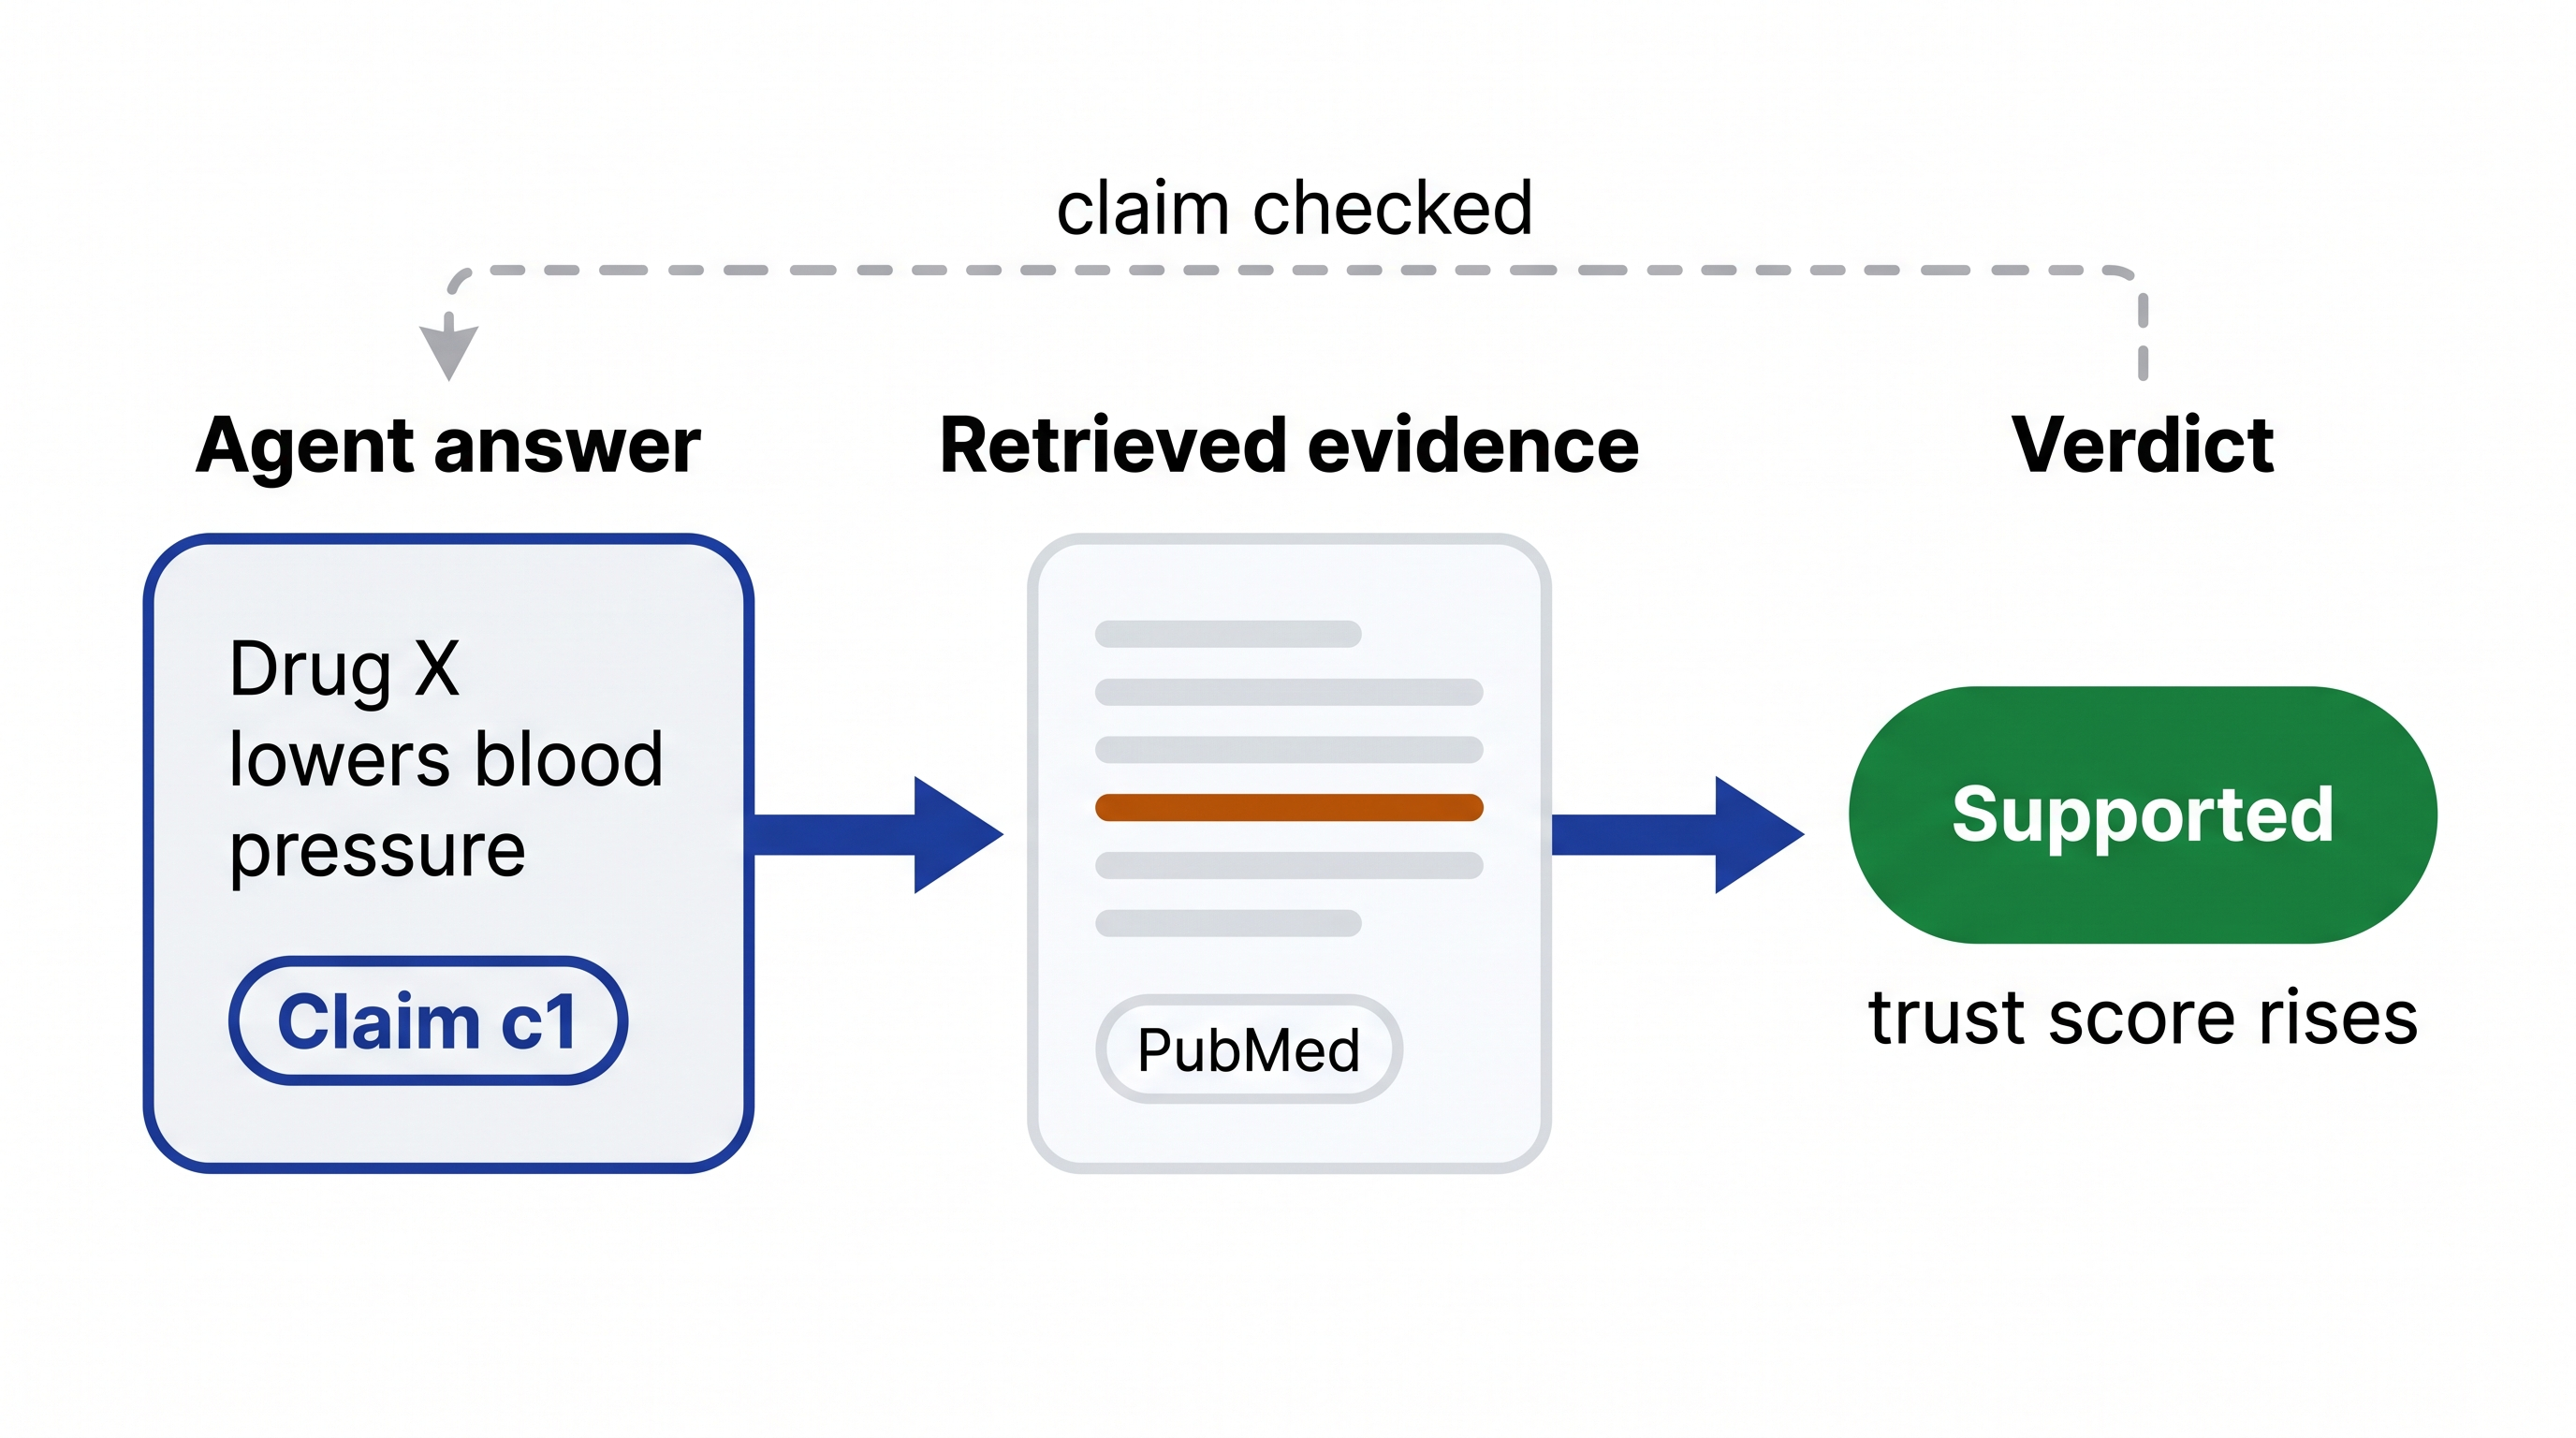
\includegraphics[width=0.80\linewidth]{fig-claim-example.png}
  \caption{Worked example of a single claim verified against a retrieved passage. The claim is marked supported, and the trust score of the agent rises for that round.}\label{fig:claim-example}
\end{figure}

\subsection{Trust Update}
The trust update converts the verdicts into a bounded influence score. Let $S_i(t)$ be the raw score of agent $i$ at round $t$. The raw score grows with the number of supported claims $V_i$ and falls with the number of contradicted claims $H_i$:
\begin{equation}\label{eq:score}
S_i(t+1) = S_i(t) + \alpha V_i - \beta H_i
\end{equation}
where $\alpha$ and $\beta$ control the gain and the loss. The raw scores are then converted into weights. A softmax maps the raw scores into positive values, a clamp keeps each value inside the interval $[0.1, 0.9]$, and a renormalization returns the weights to the simplex:
\begin{equation}\label{eq:weights}
T_i = \frac{\mathrm{clamp}(\mathrm{softmax}(S)_i, 0.1, 0.9)}{\sum_{j=1}^{N} \mathrm{clamp}(\mathrm{softmax}(S)_j, 0.1, 0.9)}
\end{equation}
The clamp prevents two failure cases. No agent is silenced by a zero weight, and no agent dominates the debate with a weight of one. The renormalization keeps the sum of the weights at one, so the final decision stays a weighted choice over the agent positions. Equations~\eqref{eq:score} and~\eqref{eq:weights} form the bounded trust update, and the whole update is a pure function of the verdict counts. Figure~\ref{fig:trust-detail} traces one update from the verdict counts to the final weights of the three agents.

\begin{figure}[pos=htbp]
  \centering
  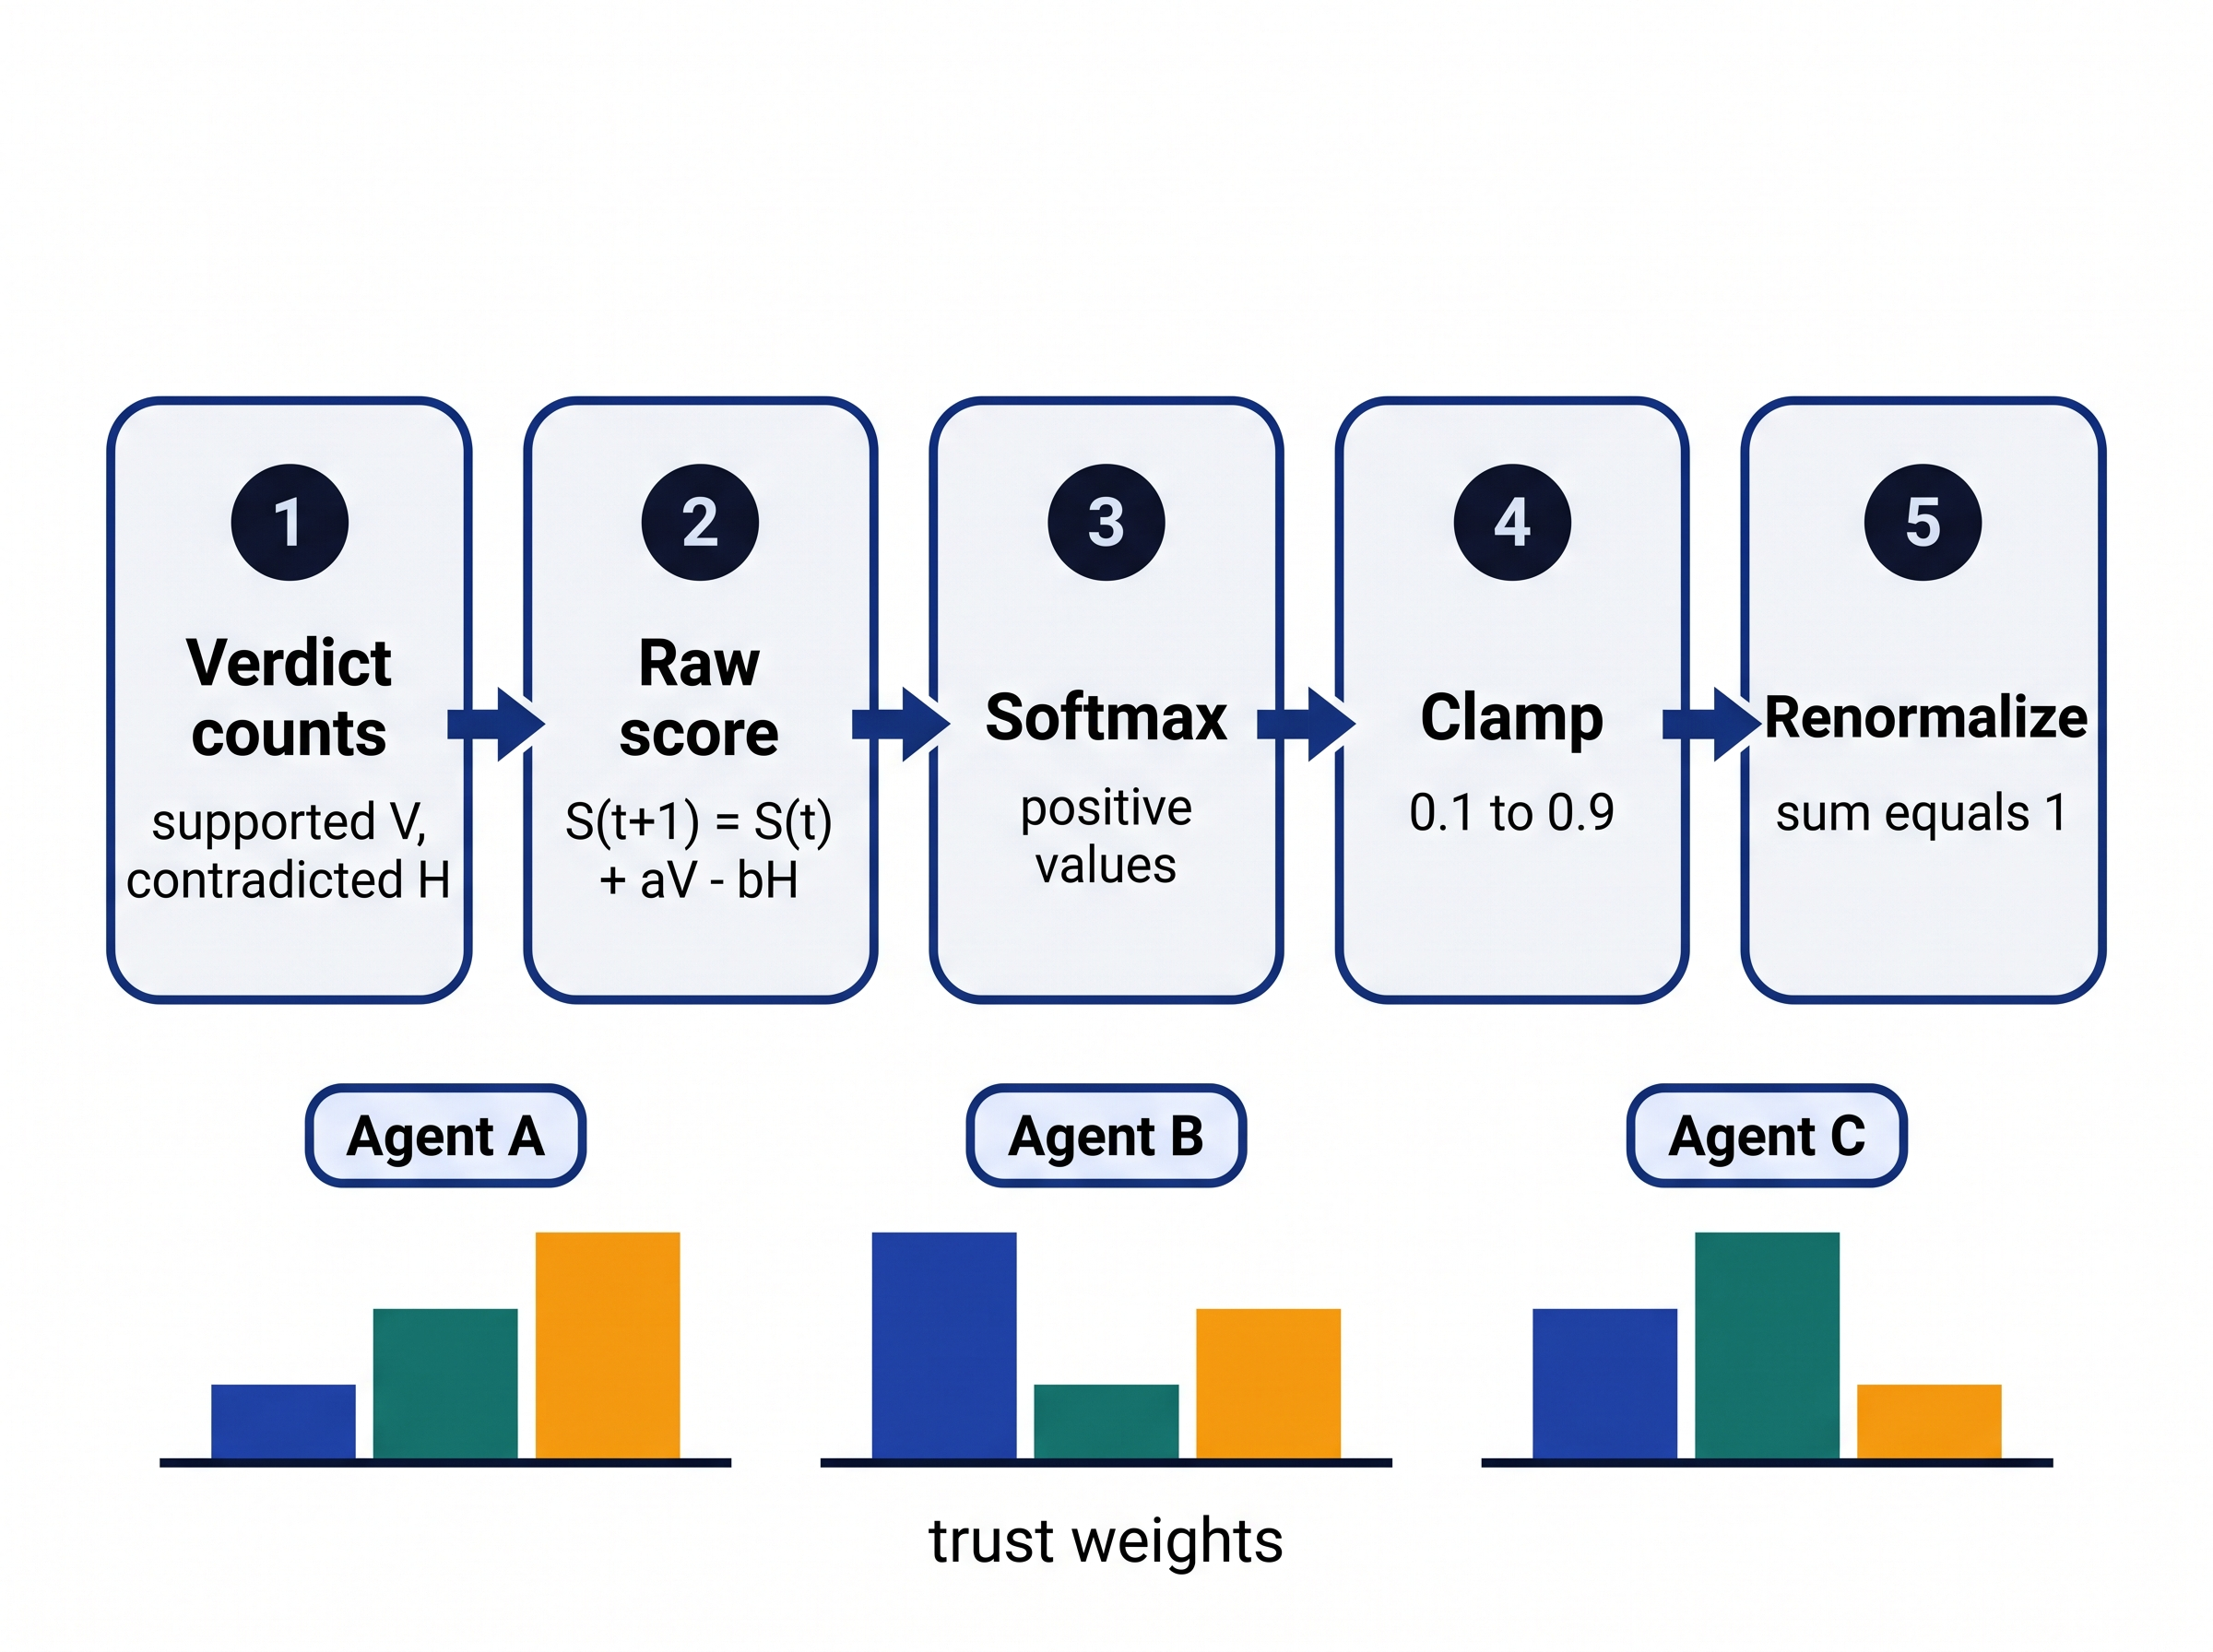
\includegraphics[width=0.58\linewidth]{fig-trust-detail.png}
  \caption{The five steps of one trust update. The verdict counts feed the raw score, and the softmax, clamp, and renormalization steps turn that score into the final trust weights of the three agents.}\label{fig:trust-detail}
\end{figure}

\subsection{Deliberation Protocol}
Each round follows the same order, namely positions, decomposition, retrieval, verdicts, and trust update. Table~\ref{tbl:rounds} lists the stages of one debated question and the number of model calls per stage. In round two and round three the revision prompt shows the agent the positions of the other agents and its own current trust value. The debate stops after round three. An injection point sits between round one and round two. At this point the evaluation harness can insert a fabricated expert consensus that contradicts a correct minority. The injection is used only in the stress tests and never in normal operation. Figure~\ref{fig:round-loop} shows the loop and where the injection enters it. A timeout or a parse failure marks the round inconclusive for that agent, and the debate continues with the remaining agents. Figure~\ref{fig:dataflow} shows the level-one data flow, including the three data stores that hold the debate state, the evidence log, and the results log.

\begin{figure}[pos=htbp]
  \centering
  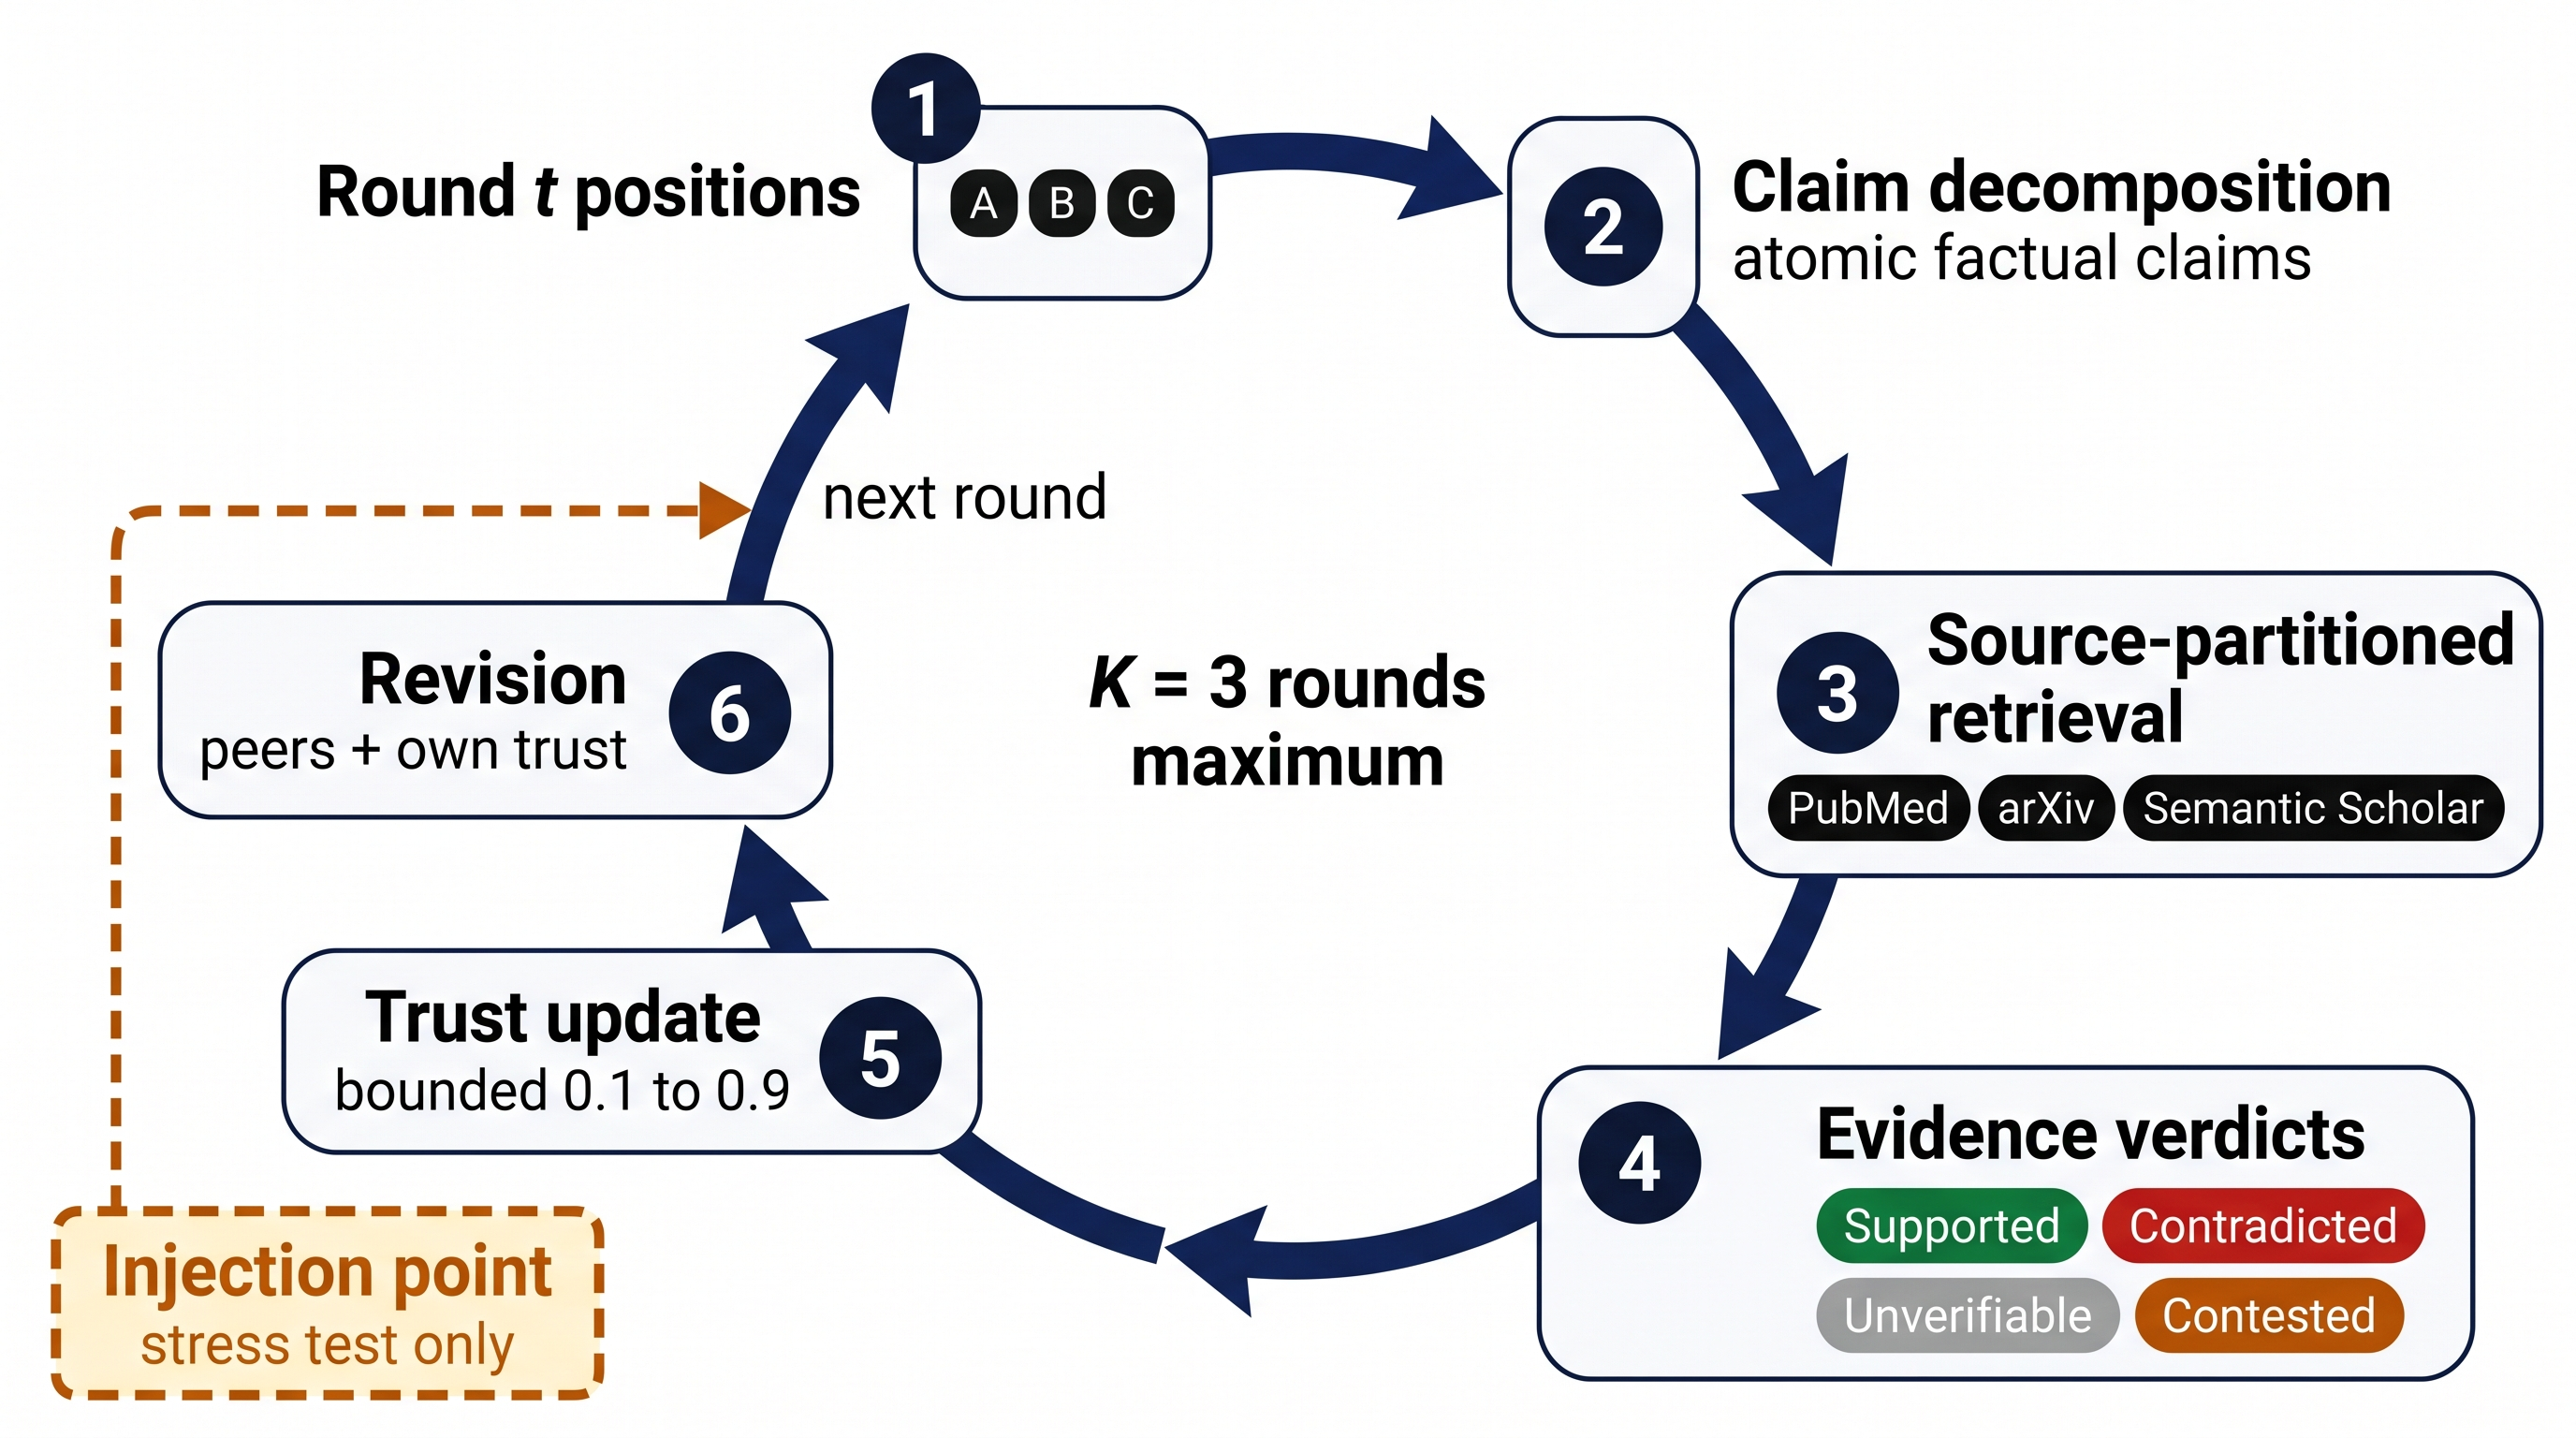
\includegraphics[width=0.88\linewidth]{fig-round-loop.png}
  \caption{The debate round loop. The six stages run in order for at most three rounds, and the injection point enters between round one and round two in the stress tests.}\label{fig:round-loop}
\end{figure}

\begin{table}
\caption{Stages of one debated question and their model calls.}\label{tbl:rounds}
\renewcommand{\arraystretch}{1.2}
\begin{tabularx}{\textwidth}{|p{4.3cm}|X|c|}
\hline
\textbf{Stage} & \textbf{What happens} & \multicolumn{1}{c|}{\textbf{Model calls}}\\
\hline
Confidence gate & Decides between a direct answer and a full debate & 1 or 3 \\
\hline
Round 1 positions & Three agents answer independently and tag their claims & 3 \\
\hline
Claim check (each round) & Decomposition, retrieval, and verdicts label every claim & 0 \\
\hline
Trust update (each round) & Verdict counts move the raw score, then the weights & 0 \\
\hline
Injection (stress tests only) & Fabricated wrong consensus enters between round 1 and round 2 & 0 \\
\hline
Round 2 revision & Agents see peer positions and their own trust, then revise & 3 \\
\hline
Round 3 revision & Final revision round, after which the debate stops & 3 \\
\hline
Aggregation & Trust-weighted answer is selected and packaged & 0 \\
\hline
\textbf{Total} & & \textbf{10} \\
\hline
\end{tabularx}
\end{table}

\begin{figure}[pos=htbp]
  \centering
  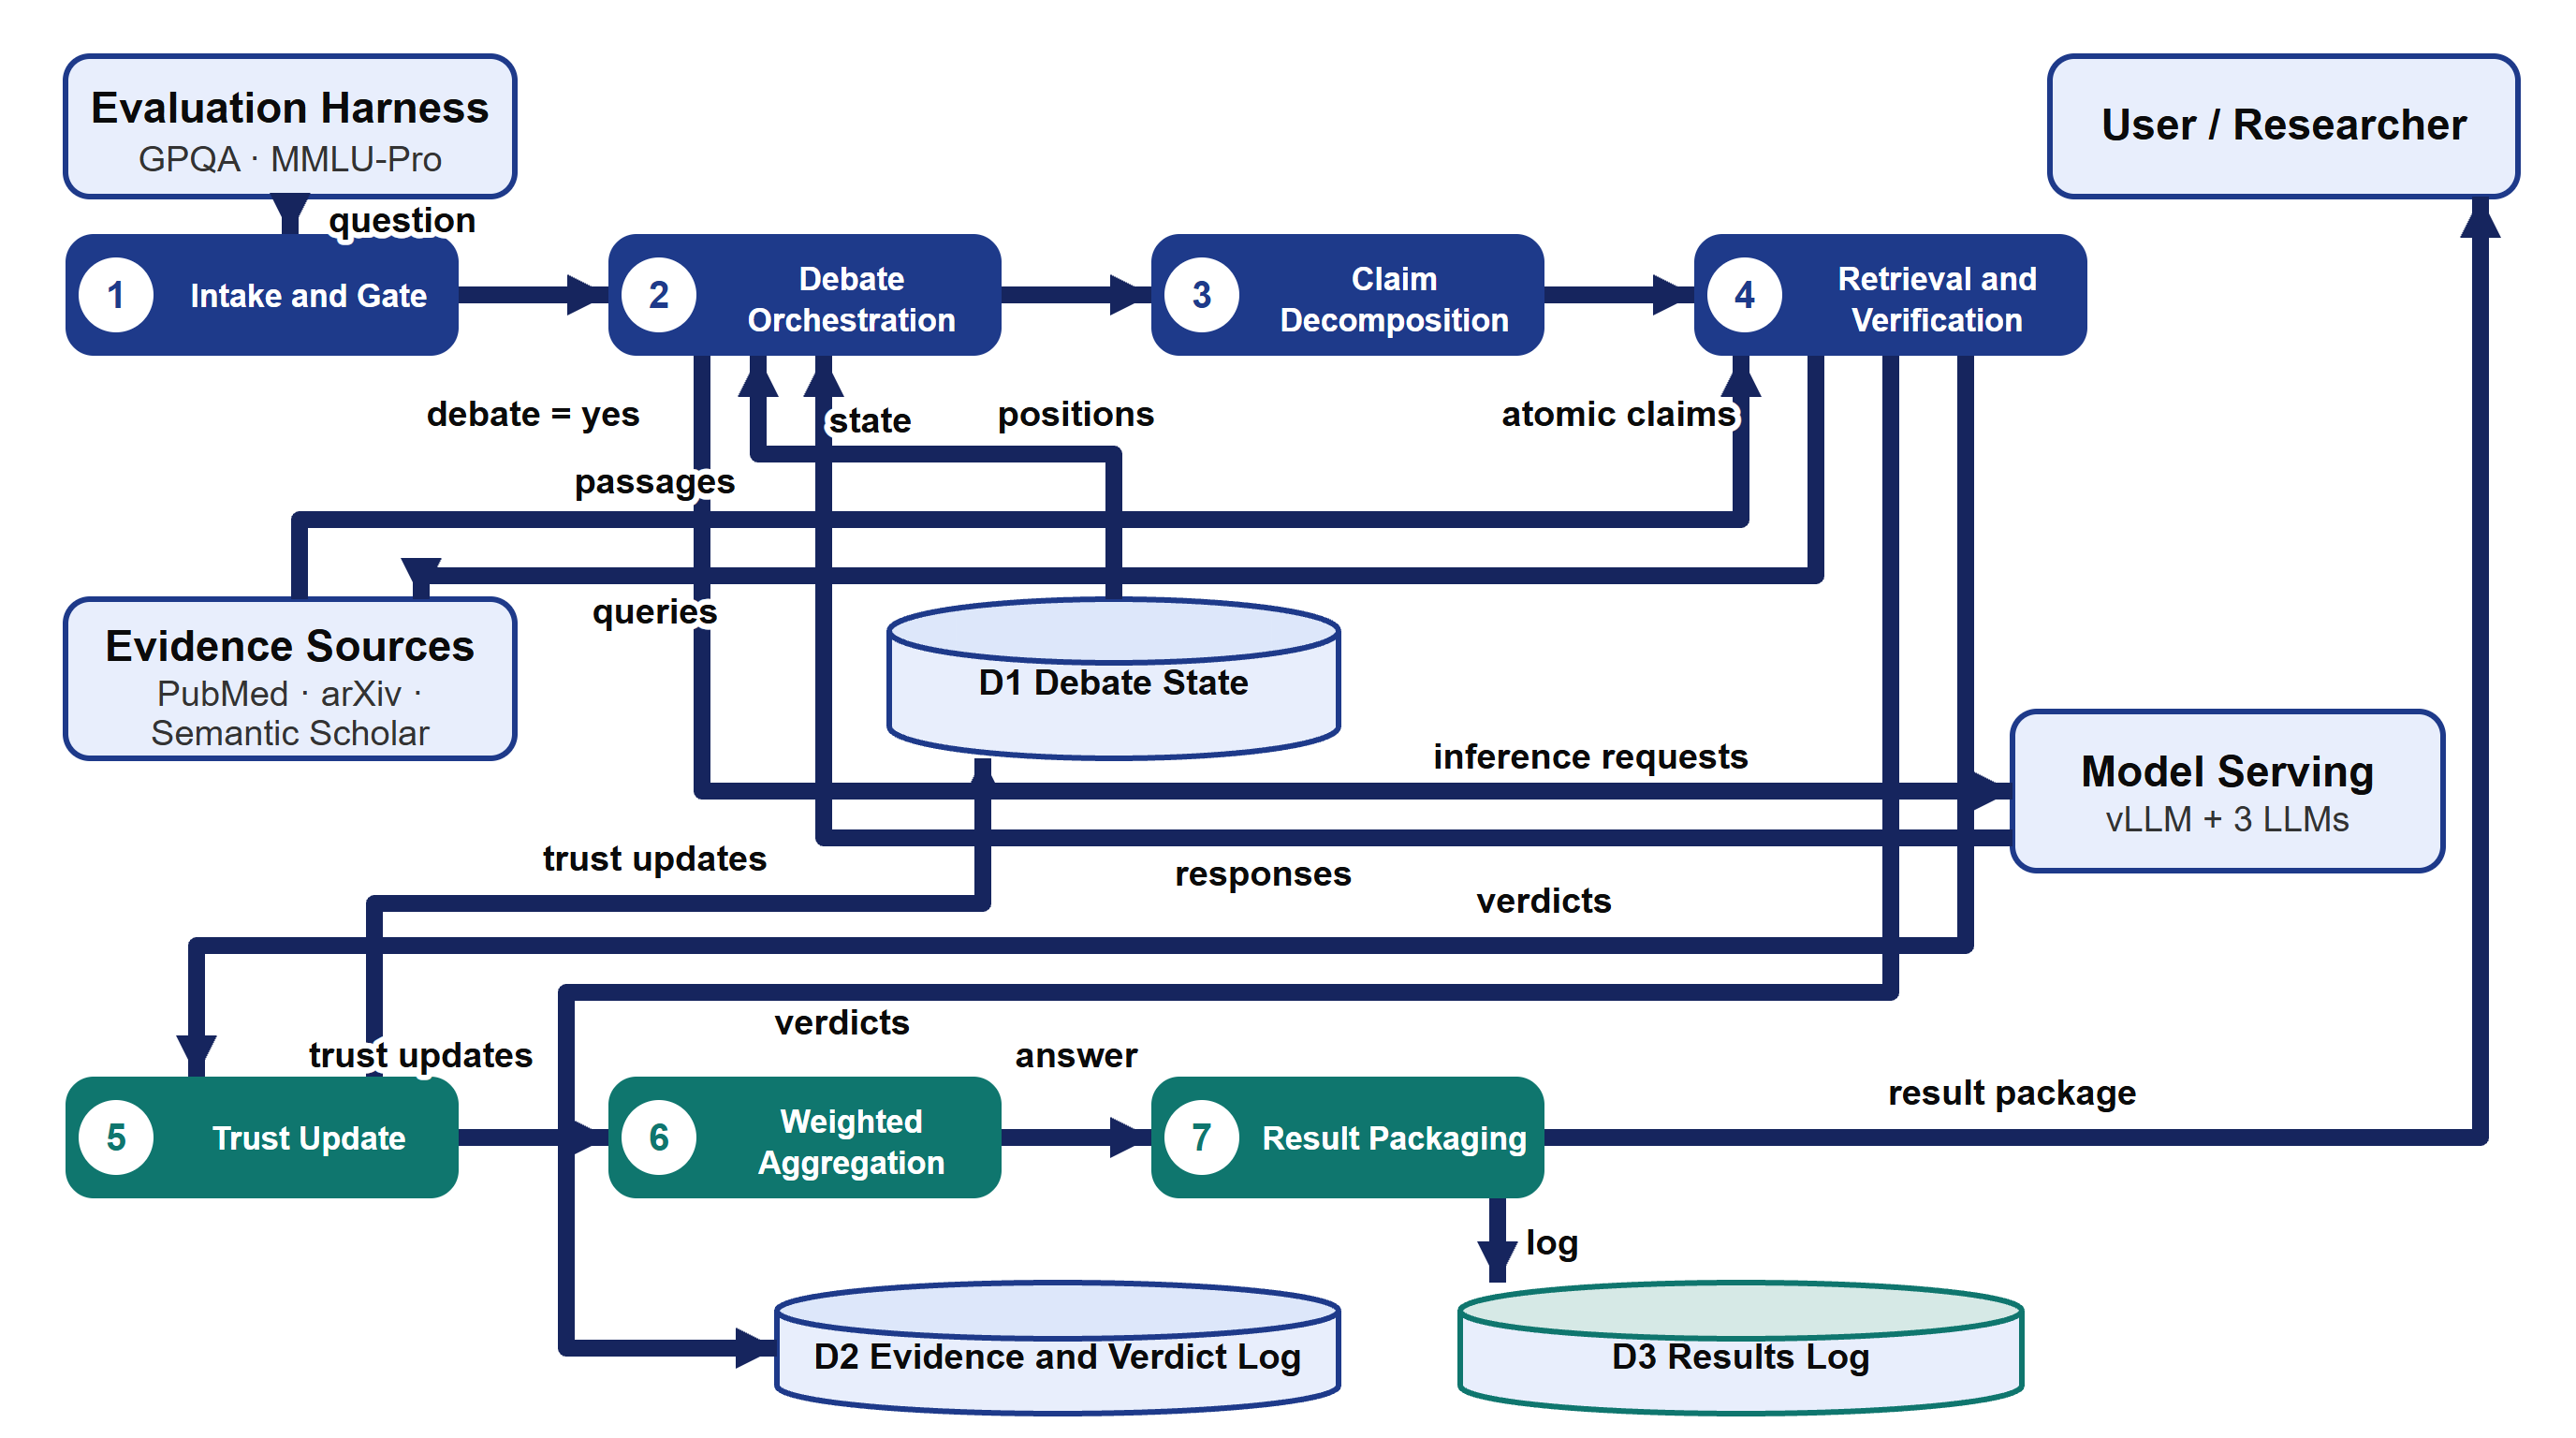
\includegraphics[width=0.88\linewidth]{fig-dataflow.png}
  \caption{Level-one data flow of the framework with the debate state, the evidence log, and the results log.}\label{fig:dataflow}
\end{figure}

\subsection{Trust-Weighted Aggregation}
The final answer is the position with the highest weighted support:
\begin{equation}\label{eq:aggregate}
a^{*} = \arg\max_{a} \sum_{i:\, p_i = a} T_i
\end{equation}
where $p_i$ is the position of agent $i$ at the last round and $T_i$ is its final trust weight. The aggregation ignores the plain head count. This is the step that allows a correct, evidence-backed minority to outweigh a wrong majority. The result package records the final answer, the evidence citations, the trust trajectory of every round, and the reasoning trace of every agent. The trajectories are stored because the evaluation uses them for the calibration analysis.

\subsection{Complexity}
A debated question uses about ten model calls. The gate uses one call, the initial round uses three calls, and the two revision rounds use three calls each. The retrieval traffic scales with the number of claims, and the cache removes repeated queries. The pipeline runs on a single rented GPU and requires no fine-tuning.

\clearpage

\section{Experiment}

\subsection{Dataset}

\section{Results}

\section{Conclusion}

\section*{Declarations}
\begin{itemize}
\item \textbf{Conflicts of Interest:}  The authors declare no conflicts of interest.

\item \textbf{Data availability:} Data will be made available on request to the corresponding
authors.
\end{itemize}
%%%%%%%%%%%%%%%%%%%%%%%%%%%%%%%
\printcredits

\newpage
\bibliographystyle{elsarticle-num}
\nocite{*}
\bibliography{cas-refs}

\vspace{12pt}
\end{document}

